\documentclass[
hidelinks,
12pt,
openany,
oneside,
a4paper,
chapter=TITLE,
portuguese, % ou english
english
]{abntex2}

\usepackage{config}
\makeglossaries

\begin{document}
\begin{OnehalfSpace}
\begin{center}
            \begin{figure}[htbp]
                \centering
                
\includegraphics[width=13cm]{assets/unologo-enhanced}
            \end{figure}
        
            \MakeUppercase{\textbf{Universidade Comunitária da Região de Chapecó}} \\
            \MakeUppercase{\textbf{ATEC - ÁREA DE ENGENHARIAS E SUAS TECNOLOGIAS}}\\
            \MakeUppercase{\textbf{CIÊNCIA DA COMPUTAÇÃO}}\\
            \MakeUppercase{\textbf{(CURSO DE CIÊNCIA DA COMPUTAÇÃO)}}\\
            
            \vspace{4.5cm}
            
            \MakeUppercase{\textbf{PROTÓTIPO DE APLICAÇÃO DE ENVIO DE DOCUMENTOS MODELADO COM C4
            MODEL, UTILIZANDO ARQUITETURA DE MICRO SERVIÇOS E MENSAGERIA}}
            
            \vspace{3.5cm}
            
            \MakeUppercase{\textbf{Felippe Butland}}
            
            \vfill
            
            \MakeUppercase{\textbf{Chapecó, Novembro de 2024}}
         
\end{center}
\clearpage

\pagenumbering{roman}
\textual
\pagestyle{simple} % tira cabeçalho com nome do capítulo e exibe só paginação
\setcounter{page}{2}
% Folha de rosto

    \begin{center}
    \vspace{1cm}
    
    \textbf{\MakeTextUppercase{Universidade Comunitária da Região de Chapecó}\\}
    \textbf{\MakeTextUppercase{ATEC - ÁREA DE ENGENHARIAS E SUAS TECNOLOGIAS}\\}
    \textbf{\MakeTextUppercase{CIÊNCIA DA COMPUTAÇÃO}\\}
    \textbf{\MakeTextUppercase{(CURSO DE CIÊNCIA DA COMPUTAÇÃO)}\\}

    \vspace{6cm}

    % \MakeUppercase{\textbf{Protótipo de plataforma de dados escalável para processamento Big Data, utilizando dados  da agricultura}}
    \MakeUppercase{\textbf{PROTÓTIPO DE APLICAÇÃO DE ENVIO DE DOCUMENTOS MODELADO COM C4
    MODEL, UTILIZANDO ARQUITETURA DE MICRO SERVIÇOS E MENSAGERIA}}

    \end{center}

    \vspace{3cm}

    \begin{flushright}
        \hspace*{7cm}
        \begin{minipage}{0.5\textwidth}

            \bfseries
            % \footnotesize
            \SingleSpacing

%                        Relatório do Trabalho de Conclusão de Curso submetido à Universidade Comunitária da Região de Chapecó para obtenção do título de bacharelado no curso de Ciência da Computação.

            			 Monografia apresentada ao Curso de Ciência da Computação, da Escola Politécnica da Universidade Comunitária da Região de Chapecó, como  parte dos requisitos para obtenção do Título de Bacharel em Ciência da Computação.\\
        
        \end{minipage}
    \end{flushright}

    \vspace{0.5cm}
    \begin{center}
    \textbf{\MakeTextUppercase{Felippe Butland}}
    \end{center}
    \vspace{0.5cm}

    {
        \hspace*{7cm}
        \begin{minipage}{0.5\textwidth}
            \mdseries
            % \footnotesize
            \SingleSpacing

            Orientador: Prof. Me. Radámes Pereira
            % \hspace*{2.3cm}\textmd{Mestre}
        \end{minipage}
    }

    \vfill

    \begin{center}
    \textbf{\MakeTextUppercase{Chapecó, Novembro de 2024}}
    \end{center}

    \OnehalfSpacing
    \begin{center}
        \ABNTEXchapterfont%

        \MakeTextUppercase{\textbf{PROTÓTIPO DE APLICAÇÃO DE ENVIO DE DOCUMENTOS MODELADO COM C4
        MODEL, UTILIZANDO ARQUITETURA DE MICRO SERVIÇOS E MENSAGERIA}}

        \vspace{2\baselineskip}

        \MakeTextUppercase{\textbf{Felippe Butland}}

        \vspace{2\baselineskip}
        
        \MakeTextUppercase{\textbf{ESTE RELATÓRIO, DO TRABALHO DE CONCLUSÃO DE CURSO, FOI JULGADO ADEQUADO PARA OBTENÇÃO DO TÍTULO DE:}}\\
        l~pç\vspace{\baselineskip}
        \MakeTextUppercase{\textbf{BACHAREL EM CIÊNCIA DA COMPUTAÇÃO} }
        
        \vspace{3\baselineskip}

        \textmd{Prof. Me. Radámes Pereira}\\
        Orientador\\
    \end{center}

    \vspace{2\baselineskip}
    \noindent
    \textbf{BANCA EXAMINADORA:}\\
   
    \vspace{3\baselineskip}

    \noindent
    \begin{minipage}{0.5\textwidth}
        \mdseries
        \SingleSpacing
        \centering

        \textmd{Ariel Zuquello}, \textmd{Prof. Dr.}\\
        \textbf{Membro da banca}
    \end{minipage}
    \hfill
    \begin{minipage}{0.5\textwidth}
        \mdseries
        \SingleSpacing
        \centering

        \textmd{Viviane D. Bonfim}, \textmd{Prof. Dr.}\\
        \textbf{Membro da banca}
    \end{minipage}\\

    \vspace{3\baselineskip}
    \noindent
    \begin{minipage}{0.5\textwidth}
        \mdseries
        \SingleSpacing
        \centering

        \textmd{Radamés Pereira}, \textmd{Prof. Me.}\\
        \textbf{Supervisor de TCC}
    \end{minipage}
    \hfill
    \begin{minipage}{0.5\textwidth}
        
            \mdseries
            % \footnotesize
            \SingleSpacing
            \centering

            \textmd{Sandro Silva de Oliveira}, \textmd{Dr.}\\
            \textbf{Coordenador de Curso}
    \end{minipage}

    \vfill
    \begin{center}
        \textmd{Chapecó, Novembro de 2024}
    \end{center}
    \clearpage
    
    % \vspace{0,5cm}
%\input{pages/3_figuras}
%\input{pages/4_quadros}
\setlength{\absparsep}{18pt} % ajusta o espaçamento dos parágrafos do resumo
\begin{resumo}
\noindent Felippe Butland\textbf{PROTÓTIPO DE APLICAÇÃO DE ENVIO DE DOCUMENTOS MODELADO COM C4
MODEL, UTILIZANDO ARQUITETURA DE MICRO SERVIÇOS E MENSAGERIA}. 2024. Trabalho de Conclusão de Curso - Ciência da Computação, Universidade Comunitária da Região de Chapecó, Chapecó, 2024.\\


\noindent  Este trabalho descreve o desenvolvimento de um protótipo de aplicação para envio de documentos utilizando uma arquitetura de microserviços, mensageria e modelagem com o C4 Model. A escolha dessa arquitetura visa oferecer modularidade e escalabilidade, atendendo às necessidades de aplicações corporativas e à realidade de startups, que frequentemente hesitam em investir em arquitetos de software devido aos custos. Foi criada uma solução baseada em microserviços separados para login, cadastro e envio de documentos, com comunicação via mensageria, o que proporcionou um sistema eficiente e resiliente para o tráfego de dados.  Os testes de benchmark realizados demonstraram que a aplicação pode lidar com um volume satisfatório de requisições, embora a segmentação em microserviços possa introduzir latência, especialmente em ambientes multi-região. Conclui-se que uma arquitetura bem planejada e documentada, mesmo com recursos limitados, permite desenvolver aplicações escaláveis e de fácil manutenção, servindo como referência para startups e pequenas empresas que buscam eficiência e sustentabilidade a longo prazo.

\noindent Palavras-chave: Micro-Serviços, C4Model, Mensageria.
\end{resumo}
% resumo em inglês
\begin{resumo}[Abstract]
 \begin{otherlanguage*}{english}
\noindent Felippe Butland  \textbf{DOCUMENT SUBMISSION APPLICATION PROTOTYPE MODELED WITH C4 MODEL, USING MICRO-SERVICES ARCHITECTURE AND MESSAGING}. 2024. Undergraduate Thesis – Computer Science, Universidade Comunitária da Região de Chapecó, Chapecó, 2024.\\

\noindent This work describes the development of a document submission prototype application using a microservices architecture, messaging, and the C4 Model for modeling. The chosen architecture aims to provide modularity and scalability, addressing the needs of corporate applications and the reality of startups, which often hesitate to invest in software architects due to cost constraints. The solution was developed with separate microservices for login, registration, and document submission, with communication via messaging, creating an efficient and resilient data traffic system.
Benchmark tests demonstrated that the application can handle a satisfactory volume of requests, although the segmentation into microservices may introduce latency, especially in multi-region environments. The conclusion is that a well-planned and documented architecture, even with limited resources, allows for the development of scalable and maintainable applications. This work serves as a reference for startups and small companies seeking efficiency and long-term sustainability.

\noindent \textbf{Keywords:} software architecture, microservices, messaging, C4 Model, startups, documentation, scalability
\end{otherlanguage*}


\end{resumo}

% Lista de ilustrações (elemento opcional - recomenda-se que sejam elaboradas a partir de 5 itens)
%\listoffigures*
%\clearpage
% Lista de tabelas (elemento opcional - recomenda-se que sejam elaboradas a partir de 5 itens)
%\listoftables*
%\cleardoublepage
% \cleardoublepage
%% Lista de abreviaturas e siglas (elemento opcional - recomenda-se que sejam elaboradas a partir de 5 itens)
\newacronym{CRM}{CRM}{Customer Relationship Management}
\newacronym{UML}{UML}{Linguagem de Modelagem Unificada}
\newacronym{SQL}{SQL}{Structured Query Language}
\newacronym{ACID}{ACID}{Atomicidade, Consistência, Isolamento e Durabilidade}
\newacronym{API}{API}{Application Programming Interface}
\newacronym{RLS}{RLS}{Row Level Security}
\newacronym{JSON}{JSON}{JavaScript Object Notation}
\newacronym{JWT}{JWT}{JSON WEB Token}
\newacronym{CLI}{CLI}{interface de linha de comando}
\newacronym{URL}{URL}{Uniform Resource Locator}
\newacronym{NPM}{NPM}{Node Package Manager}
\printglossary[type=\acronymtype, title=LISTA DE ABREVIATURAS]
\clearpage


% Lista de abreviaturas e siglas (elemento opcional - recomenda-se que sejam elaboradas a partir de 5 itens)

\pdfbookmark[0]{\bfseries\fontfamily{ptm}\selectfont\contentsname}{toc}
\tableofcontents*
\cleardoublepage

\pagenumbering{arabic}
\chapter{INTRODUÇÃO}
A arquitetura de software é um processo complexo e dinâmico. Conforme Martin (2020)
afirma, "uma arquitetura bem definida é um processo contínuo de investigação, e não um artefato
congelado". Ou seja, trata-se de um estudo contínuo e análise profunda do software, bem como
das definições e previsões futuras. Esse processo é condicionado a uma operação constante, em
que todos os envolvidos no software devem estar alinhados com as tecnologias e as definições
do profissional responsável pela arquitetura e definições técnicas do software. Esse processo
de desenhar, planejar e construir uma aplicação é contínuo e envolve decisões críticas para
o software. Muitas vezes, é referido como design de software, pois envolve a definição de
componentes e conectores entre as aplicações do sistema. Além disso, é necessário estabelecer
padrões de sistema, como a arquitetura em camadas, orientada a eventos, entre outras. Para
arquitetar um software, é fundamental ter uma visão de longo prazo, prevendo futuras abordagens
e qualidades do software.

\section{Contextualização}
A definição das arquiteturas para aplicações torna-se cada vez mais complexa, pois muitas
decisões iniciais podem não estar claras, como a quantidade de acessos e o público-alvo. No
entanto, é possível definir aspectos importantes desde o início, como se a comunicação será
síncrona ou assíncrona, e onde os dados serão armazenados. Para isso, é necessário arquitetar,
modelar e redesenhar o sistema várias vezes até que atenda às expectativas do arquiteto ou às
necessidades do produto.

\section{Delimitação do problema}

A implementação de uma arquitetura robusta de software pode ser um desafio financeiro,
onde o papel do arquiteto de software está mais voltado para a concepção da aplicação e não gera
lucro direto. Considerando isso, o objetivo deste trabalho é destacar a importância crítica e a ne-
cessidade de uma arquitetura de software apropriada para o desenvolvimento de um protótipo de
aplicação de envio de documentos, com foco em uma arquitetura de micro serviços, mensageria
e modelando com C4 Model. Além disso, essa pesquisa pretende examinar e incorporar modelos
de arquitetura sugeridos por profissionais da comunidade e por cientistas proeminentes da área,
visando simplificar a procura por soluções e minimizar os gastos relacionados à arquitetura de
software. O estudo também tem como meta entender as razões que levam startups a hesitar em
investir em arquitetos de software, fornecendo um modelo econômico e eficaz para a aplicação
de envio de documentos.

\section{Objetivos}

\subsection{Objetivo geral}
Desenvolver o protótipo de aplicação utilizando arquitetura de micro serviços, mensageria
e modelagem com C4 model.

\subsection{Objetivos específicos}
\begin{itemize}
    \item Desenvolver orientado à arquitetura de software utilizando a modelagem C4 Model;
    \item Explorar técnicas e tecnologias modernas para o desenvolvimento;
\end{itemize}

\section{Justificativa}
A medida que o volume de documentos digitais aumenta exponencialmente nas empresas
e instituições, torna-se cada vez mais crítico possuir um sistema eficiente de envio de documentos.
Além disso, a crescente demanda por escalabilidade, disponibilidade e confiabilidade nos sistemas
de TI torna a arquitetura de micro serviços, mensageria e modelagem com C4 Model uma escolha
apropriada para o desenvolvimento desta aplicação.

O uso da arquitetura de micro serviços permitirá modularizar a aplicação, separando as
funções e responsabilidades em serviços independentes. Isso facilita a manutenção e escalabi-
lidade do sistema, além de garantir maior resiliência, já que a falha de um serviço não afeta a
operação dos outros.

A inclusão da mensageria na arquitetura auxilia na comunicação assíncrona entre os
micro serviços, permitindo um maior desacoplamento entre eles. Esse desacoplamento garante
uma melhor distribuição de carga e uma resposta mais rápida às mudanças, tanto em termos de
volume de tráfego quanto de alterações nos requisitos do sistema.

O uso do C4 Model, que é uma estrutura para visualização da arquitetura de software,
oferece uma maneira clara e intuitiva de descrever e comunicar a estrutura do sistema. Essa
abordagem melhora a colaboração entre os membros da equipe, permitindo uma compreensão
comum da arquitetura e facilitando a tomada de decisões de design.

A proposta deste trabalho é desenvolver um protótipo de uma aplicação que seja escalável,
resiliente e de fácil manutenção, que se beneficie das vantagens das tecnologias de micro
serviços, mensageria e C4 Model, e que possa eficientemente gerenciar e realizar o envio de
documentos. Considerando as necessidades crescentes das empresas para gerir grandes volumes
de documentos digitais, acredita-se que este trabalho terá um impacto significativo na eficiência
das operações de TI e na produtividade geral das organizações.

\section{Procedimentos metodológicos}
O trabalho inicia com a definição clara do problema e das necessidades que a aplicação
de envio de documentos deverá resolver. Isso envolve o alinhamento das expectativas, limitações,
desafios e objetivos do projeto.
Com o problema definido, prosseguimos para a modelagem dos dados usando o C4 Model.
Nesta etapa, são criados diagramas para visualizar a arquitetura da aplicação em diferentes níveis
de abstração, desde o contexto do sistema até os componentes individuais.
Baseando-se na modelagem de dados, identificamos as estruturas de micro serviços
necessárias e as comunicações entre eles. Este procedimento também engloba a definição da
formatação e dos estilos de comunicação que serão empregados.
Com os micro serviços e as comunicações definidos, começamos o desenvolvimento do
protótipo da aplicação. Garantimos que os micro serviços sejam bem definidos e capazes de se
comunicarem eficientemente.
Em seguida, implementamos a mensageria, um método de comunicação entre os micro
serviços. Escolhemos uma plataforma de mensageria adequada, com o Kafka, a configuramos e
a integramos aos micro serviços.
Depois da implementação, testamos a aplicação para garantir que o fluxo de envio de
documentos funciona conforme o esperado. Os testes podem incluir testes unitários, de integração
e de carga. Baseando-se nos resultados, realizamos os ajustes necessários.
Por fim, documentamos todo o processo, desde a definição do problema até os testes e
ajustes. A documentação descreve como a aplicação foi modelada, quais micro serviços foram
utilizados, como a mensageria foi implementada, e os resultados dos testes.


\section{Estrutura do trabalho}
Neste capítulo foram apresentados tópicos sobre arquitetura de software e introdução
acerca do trabalho e do conteúdo, nos próximos capítulos, citamos a revisão bibliográfica e eixos
norteadores do trabalho.
\chapter{Revisão bibliográfica}
Este capítulo aborda as teorias e conceitos que foram necessários para a realização da
pesquisa. Será elaborado uma revisão dos principais tópicos que explicam um melhor entendi-
mento sobre o amplo conceito de arquitetura de software e quais arquiteturas utilizaremos neste
trabalho.


\section{Arquitetura de micro serviços}
A Arquitetura de sistemas é um processo desafiador e crucial, principalmente em startups
que precisam lançar o produto o mais rápido possível. É de extrema importância também para
organizações que desejam melhorar, ou garantir, a eficiência, segurança e manutenção de seus
sistemas. Segundo \cite{Martin2017}, "a arquitetura é o conjunto de decisões que você queria ter
tomado logo no início de um projeto, mas, como todo mundo, não teve imaginação necessária".
Além disso, o crescimento do mercado, cria oportunidades para profissionais especializa-
dos nessa área. Com o crescimento do mercado, também as empresas buscam mais competitivi-
dade, lucratividade, com um software bem arquitetado, podemos garantir um custo mais baixo,
na implementação de novas funcionalidades, nos custos de Cloud e também de novos produtos.

Arquitetura de software é um conceito bem antigo, porém, nos últimos anos, houve
uma crescente demanda sobre a posição de Arquitetos de Solução nas empresas, muitas vezes
trabalhando como profissionais multidisciplinares, arquitetam, desenvolvem Designs System,
criam a documentação, e por muitas vezes, atuam também como líderes técnicos de times de
desenvolvimento.

Gigantes da tecnologia, que também são startups, muitas vezes compartilham suas
arquiteturas através da internet, para as pessoas terem conhecimento da complexidade do sistema
deles, como a imagem abaixo ilustra, a arquitetura de processamento de pagamento da Uber:
É um tema complexo e abrangente, discutido abertamente entre as pessoas técnicas e as
mais diversas corporações no mundo inteiro, além de ser necessário para todas as aplicações,
claramente, se a aplicação não tem um grande retorno financeiro ou uma grande complexidade,
não se tem a necessidade de ter um profissional especializado ou exclusivo para esse tema, porém,
é de extrema importância ter um profissional com experiência ou conhecimento técnico no time.
Obviamente, há diversos modelos de arquitetura desenvolvidos pela comunidade, ou
por grandes profissionais da computação em uso atualmente. Cada dia mais vem surgindo
novos modelos de arquitetura para satisfazer as necessidades de projetos. Para esse trabalho, por
exemplo, utilizaremos mais de um padrão arquitetural, a fim de abordar uma arquitetura ideal
para o projeto proposto.

É definido por \cite{Newman2015}, é uma abordagem que divide uma aplicação em
pequenos serviços independentes, cada um com uma única responsabilidade e modelado em
torno de um domínio de negócios. Esses serviços autônomos trabalham juntos e podem ser
desenvolvidos, implantados e escalados de maneira independente, o que facilita a modularidade,
melhorando a manutenção e o desenvolvimento do sistema.

\begin{figure}[!ht]
    \centering
    \caption{Arquitetura de micro-serviços}
    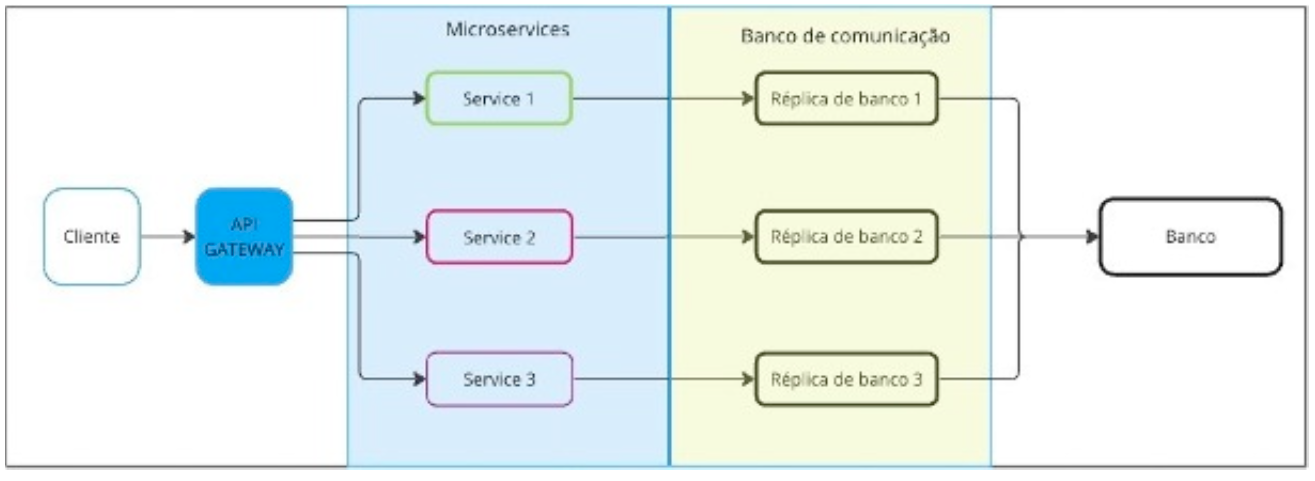
\includegraphics[scale=0.44]{assets/ms-arch}
    \label{fig:ms-arch}
    \tiny
    \sourcemedaddy
\end{figure}

Este modelo arquitetônico surgiu para solucionar desafios relacionados à escalabilidade,
eficiência, velocidade de desenvolvimento e acoplamento que são comumente encontrados em
arquiteturas monolíticas. Na arquitetura de micro serviços, cada serviço possui uma independên-
cia que garante a continuidade do funcionamento do sistema mesmo se um serviço individual
estiver indisponível \cite{Microsoft2023}.

A comunicação entre micro serviços é geralmente implementada através de APIs REST-
ful, que são baseadas em HTTP e aproveitam a infraestrutura da web \cite{LewisFowler}. No
entanto, em situações em que a latência é uma preocupação, outros protocolos de comunicação,
como o gRPC, podem ser usados.
Além disso, em operações que não exigem uma resposta
imediata, a comunicação pode ser assíncrona, com a utilização de sistemas de mensagens como
RabbitMQ ou Kafka \cite{Boner2019}.
Segundo a Microsoft, alguns dos benefícios sobre
essa arquitetura são:

\begin{itemize}
    \item \textbf{Agilidade:} ao ter um sistema quebrado em pequenos serviços, é mais ágil gerenciar correção de bugs, lançamento de recursos, além de poder reverter uma atualização se algo der errado;
    \item \textbf{Equipes pequenas e focadas:} um micro serviço deve ser pequeno o suficiente para apenas uma equipe mantê-lo, deixando a comunicação e desenvolvimento mais ágil, tendo em vista que equipes grandes tendem a ser menos produtivas, pois a comunicação é lenta e depende demais de gerenciamento;
    \item \textbf{Base de código pequena:} ao termos uma codebase, ou base de código, pequena, as dependências de código ficam menos emaranhadas, com um encapsulamento menor e menos dependências externas;
    \item \textbf{Mistura de tecnologia:} como os serviços são independentes, cada um pode ter uma linguagem de programação diferente, utilizando uma tecnologia que se adapta ao serviço melhor;
    \item \textbf{Isolamento de falhas:} se um micro serviço individual fica indisponível, ele não interrompe todo o aplicativo, desde que projetados para lidar com falhas, utilizando alguns padrões, como Circuit Breaker, ou se comunicando assincronamente;
    \item \textbf{Escalabilidade:} os serviços podem ser dimensionados independentemente, utilizando Kubernetes ou Service Fabric, por exemplo, você pode dimensionar subsistemas que exigem mais recursos;
    \item \textbf{Isolamento de dados:} é mais simples realizar atualizações de esquema, e apenas um único micro serviço é afetado, diferente de um monólito onde um todo é afetado.
\end{itemize}

Porém, temos também algumas desvantagens e/ou desafios ao implementar essa arquite-
tura, assim como:

\begin{itemize}
    \item \textbf{Complexidade:} para algumas aplicações, você implementa uma complexidade não necessária;
    \item \textbf{Desenvolvimento e testes:} as ferramentas existentes nem sempre são projetadas para funcionar com dependências de serviço. A refatoração entre limites de serviço pode ser difícil;
    \item \textbf{Falta de governança:} a abordagem descentralizada pode trazer problemas, principalmente se você tem diversas linguagens e uma gestão também descentralizada;
    \item \textbf{Integridade de dados:} como cada micro serviço é responsável pela sua própria persistência de dados, a consistência dos dados pode ser um dos desafios;
    \item \textbf{Gestão:} para desenvolver uma aplicação com grandes quantidades de serviços, deve-se ter uma cultura de DevOps madura, e os registros devem correlacionar várias chamadas de serviço para uma única operação de usuário.
\end{itemize}

Embora o uso de micro serviços ofereça muitos benefícios, também há desafios e desvan-
tagens, como a complexidade adicional para coordenação de serviços e a necessidade de uma
infraestrutura robusta para gerenciamento e monitoramento \cite{OReilly2018}.

Grandes empresas como a Netflix e a Amazon adotaram a arquitetura de micro serviços
para lidar com seus volumes massivos de transações e permitir a implantação contínua de
novos recursos \cite{BLOG2015}. No entanto, cada implementação tem suas
peculiaridades e, em alguns casos, como o da Amazon Prime Video, a migração para uma
arquitetura mais monolítica foi considerada mais benéfica \cite{Targett2023}.

\begin{figure}[!ht]
    \centering
    \caption{Arquitetura de micro-serviços AWS}
    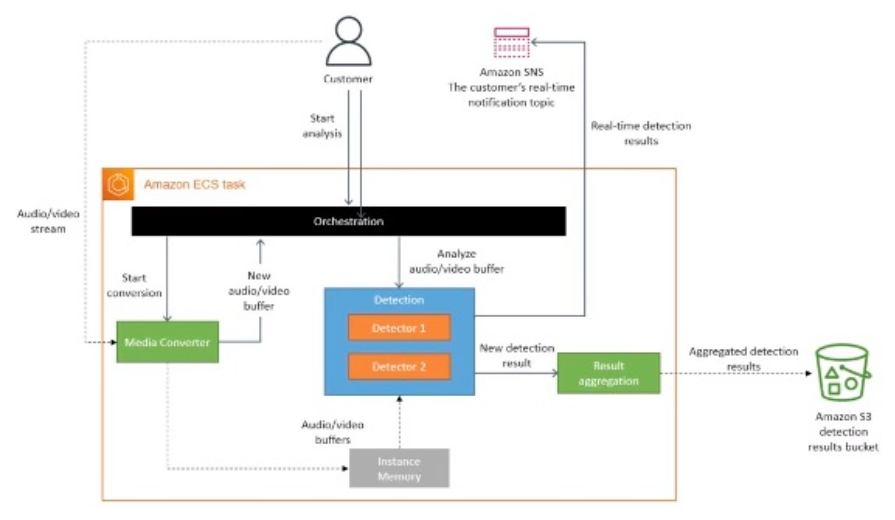
\includegraphics[scale=0.44]{assets/aws-ms}
    \label{fig:aws-ms}
    \tiny
    \sourcemedaddy
\end{figure}

Conforme imagem acima, a nova arquitetura, não foi migrada totalmente para monolito,
porém, conforme supracitado, já foi o suficiente para reduzir significativamente o custo de cloud;
por isso, deve-se tomar cuidado em abordagens como esta, pois, conforme ganha escala, o custo
fica mais caro.

Vale ressaltar que a adoção bem-sucedida de microserviços pode impactar significati-
vamente o desempenho e a escalabilidade dos sistemas \cite{Dragoni2017}. Portanto, é
crucial ponderar os benefícios e desafios antes de decidir por esta arquitetura.


\section{Arquitetura de mensageria}

A arquitetura de mensageria é uma das estratégias mais eficazes para gerenciar comuni-
cações entre serviços em um sistema distribuído, como os construídos com micro serviços.
Ela implementa comunicações assíncronas entre sistemas, geralmente recorrendo a tecnologias de
fila para garantir a entrega e o processamento de mensagens \cite{Boner2019}.

O paradigma de mensageria proporciona alta disponibilidade e resiliência, pois, mesmo que um serviço esteja temporariamente indisponível, as mensagens enviadas para ele serão armazenadas na fila até que o serviço esteja operacional novamente.
Essa característica é fundamental para sistemas de alta performance e pode minimizar o impacto de falhas em partes individuais do sistema.

Além disso, essa abordagem facilita a comunicação entre serviços escritos em diferentes linguagens de programação, uma vez que a interface de comunicação é estabelecida por meio da troca de mensagens, em vez de chamadas de método diretas.
Isso ajuda a alcançar uma verdadeira independência de serviço, que é um dos princípios fundamentais da arquitetura de micro serviços \cite{Newman2015}.

Entretanto, apesar de suas vantagens, a arquitetura de mensageria também apresenta desafios.
Um deles é a complexidade adicional na orquestração de mensagens e na gestão das filas.
Outro desafio é a dificuldade de implementar operações que exigem sincronia imediata, uma vez que a natureza assíncrona da arquitetura de mensageria pode levar a latências na comunicação \cite{Mota2022}.

Para lidar com esses desafios, algumas soluções de middleware de mensagens, como
RabbitMQ, ActiveMQ e Kafka, fornecem recursos avançados, como garantias de entrega, suporte
para padrões de mensagens complexos e mecanismos para lidar com mensagens em caso de
falha no processamento \cite{Kleppmann2017}.

Portanto, ao projetar uma arquitetura de micro serviços, a arquitetura de mensageria é uma
estratégia importante a ser considerada.
Ela fornece uma maneira de lidar com as complexidades da comunicação entre serviços, oferecendo um alto nível de desacoplamento, escalabilidade e resiliência.

Essa arquitetura é utilizada também com webhooks, e arquitetura também orientada a
eventos, quando sistemas precisam abrir uma comunicação bidirecional, como por exemplo:
temos uma criação de um Lead em um CRM e ele precisa me retornar e esperamos o retorno, logo, aguardamos o evento para uma trativa, podemos ter uma comunicação bidirecional.

Segundo \cite{LewisFowler}, algumas vantagens de utilizar mensageria são:

\begin{itemize}
    \item \textbf{Assincronismo:} a aplicação produtora da mensagem não precisa se preocupar com a aplicação consumidora estar ativa, pois o Message Broker, API Gateway ou a fila se responsabiliza em entregar quando a aplicação fica ativa novamente;
    \item \textbf{Acoplamento:} baixo acoplamento na integração entre sistemas, deixando-a assíncrona;
    \item \textbf{Múltiplas linguagens:} é possível integrar sistemas com diferentes linguagens, utilizando-as em suas especialidades.
\end{itemize}

\textbf{Desvantagens de utilizar esse modelo arquitetural:}

\begin{itemize}
    \item \textbf{Complexidade:} por ter uma certa distribuição e poder ter múltiplas linguagens, pode haver uma complexidade no desenvolvimento e manutenção do sistema;
    \item \textbf{Sincronismo:} não é adequado para cenários que exigem sincronismo entre as aplicações.
\end{itemize}

\begin{figure}[!ht]
    \centering
    \caption{Comunicação de mensageria}
    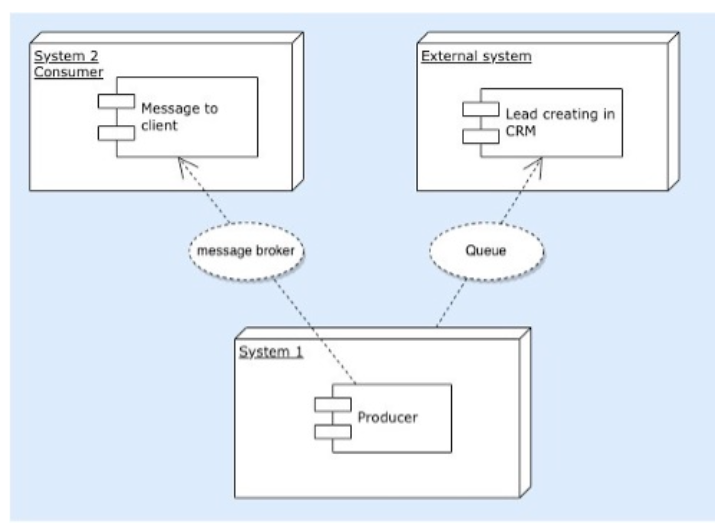
\includegraphics[scale=0.44]{assets/message-communication}
    \label{fig:message-communication}
    \tiny
    \sourcemedaddy
\end{figure}

\section{Arquitetura C4 model}
O modelo C4 é uma abordagem inovadora para a visualização da arquitetura de software.
Como mencionado anteriormente, ele foi criado por Simon Brown entre 2006 e 2011, com
o objetivo de superar as falhas na documentação e comunicação da arquitetura de software \cite{Brown2020}.

A arquitetura C4 model, ou apenas C4, consiste em uma forma ágil, com apelo téc-
nico para documentação da arquitetura de software e da parte técnica do sistema.
Segundo \cite{Santana2021} ela tem como premissa evitar dois principais cenários:

\begin{itemize}
    \item \textbf{Documentação de arquiteturas complexas:} documentações que demoram muito tempo para serem desenvolvidas ou que são difíceis de atualizar, com o tempo se tornam inutilizáveis ou obsoletas;
    \item \textbf{Documentações com poucas informações:} documentações pouco descritivas, com informações vagas ou falhas, também se tornam inutilizáveis.
\end{itemize}

O modelo C4 é baseado em quatro níveis de abstração, cada um dos quais visa um
público diferente e oferece um nível de detalhamento diferente. Isso torna o modelo C4 uma
ferramenta eficaz para a comunicação com diferentes partes interessadas, desde os não técnicos até os desenvolvedores de software \cite{Santana2021}.

O primeiro nível, o diagrama de contexto, proporciona uma visão de alto nível do sistema
em seu ambiente e é útil para comunicar a visão geral do sistema para todas as partes interessadas,
incluindo as não técnicas.
Este diagrama ilustra como o sistema interage com outros sistemas e usuários \cite{Brown2020}.

\begin{figure}[!ht]
    \centering
    \caption{Contexto C4 Model}
    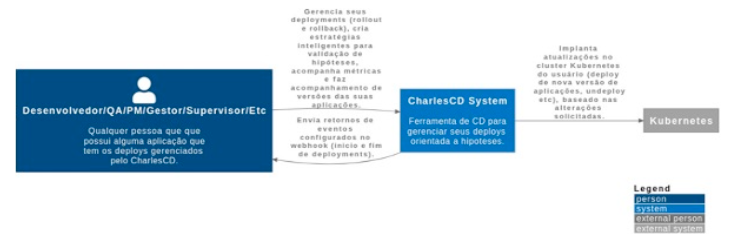
\includegraphics[scale=0.44]{assets/c4-context}
    \label{fig:c4-context}
    \tiny
    \sourcemedaddy
\end{figure}

O segundo nível, o diagrama de contêiner, é voltado para os desenvolvedores e outros
profissionais técnicos e mostra os principais componentes de alto nível do sistema, como bancos
de dados, servidores web, serviços de back-end e front-ends da web ou móveis, bem como suas
interações \cite{Brown2020}.

\begin{figure}[!ht]
    \centering
    \caption{Containers C4 Model}
    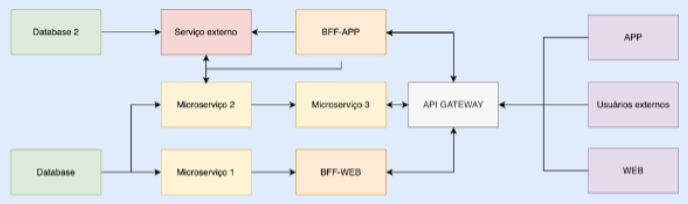
\includegraphics[scale=0.44]{assets/c4-containers}
    \label{fig:c4-containers}
    \tiny
    \sourcemedaddy
\end{figure}

O terceiro nível, o diagrama de componente, detalha ainda mais a estrutura interna de
cada contêiner, mostrando os diferentes componentes de software dentro de cada contêiner e
como eles interagem.
Este diagrama é útil para os desenvolvedores que trabalham no sistema \cite{Brown2020}.

\begin{figure}[!ht]
    \centering
    \caption{Componentes C4 Model}
    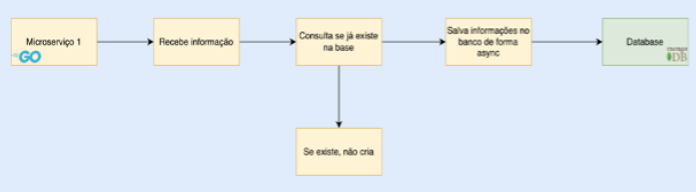
\includegraphics[scale=0.44]{assets/c4-components}
    \label{fig:c4-components}
    \tiny
    \sourcemedaddy
\end{figure}

Finalmente, o quarto nível, o diagrama de código, fornece uma visão detalhada de
algumas partes do código que são críticas para entender a implementação de determinados
componentes.
Este é o nível mais detalhado e é normalmente utilizado apenas quando necessário, devido à complexidade e ao esforço necessário para mantê-lo atualizado \cite{Brown2020}.

O modelo C4 é uma abordagem eficaz para documentar a arquitetura de software, pois
ajuda a comunicar a visão de alto nível e os detalhes técnicos de um sistema para diferentes
públicos.
No entanto, como qualquer ferramenta, ela deve ser usada adequadamente para ser
eficaz.
Isso significa que os diagramas devem ser mantidos atualizados à medida que o sistema
evolui e que o nível de detalhe deve ser adequado ao público-alvo \cite{Santana2021}.

\section{Node.JS/NestJS}

Node.js é um ambiente de tempo de execução de código aberto que permite a execução de
JavaScript no lado do servidor. Introduzido em 2009, o Node.js revolucionou o desenvolvimento
web ao permitir que os desenvolvedores criem aplicativos escaláveis e de alto desempenho
usando JavaScript tanto no cliente quanto no servidor.

De acordo com \cite{Silva2018}, o Node.js é construído com base
no mecanismo de JavaScript V8 do Google Chrome, o que o torna extremamente eficiente e
rápido. Ele usa um modelo de E/S não bloqueante, o que significa que é capaz de lidar com várias
solicitações simultaneamente, tornando-o ideal para aplicativos em tempo real, APIs RESTful e
outras aplicações de alto desempenho.

Nest.js, por sua vez, é um framework para Node.js construído com base no TypeScript.
Conforme mencionado por \cite{Tavares2020}, o Nest.js oferece uma arquitetura escalável e
modular que ajuda os desenvolvedores a criar aplicativos robustos e bem estruturados.
Ele usa conceitos familiares de outros frameworks populares, como Angular, tornando-o fácil de aprender
e usar para aqueles familiarizados com essas tecnologias.

De acordo com \cite{Johnson2020}, o Nest.js também enfatiza o uso de injeção de depen-
dência, o que facilita a criação de aplicativos altamente testáveis e extensíveis. Ele fornece um
sistema de módulos que ajuda a organizar e reutilizar o código de maneira eficiente, permitindo o
desenvolvimento de aplicativos complexos de forma mais gerenciável. Um aspecto importante do
Node.js e do Nest.js é o seu rico ecossistema de pacotes e bibliotecas. De acordo com (SANTOS,
2019), a comunidade em torno do Node.js contribuiu com uma ampla gama de módulos que
podem ser facilmente integrados aos projetos, facilitando o desenvolvimento de funcionalidades
avançadas.

\section{Typescript}

TypeScript é uma linguagem de programação de código aberto desenvolvida pela Micro-
soft que estende o JavaScript adicionando recursos de tipagem estática. Lançado em 2012, o
TypeScript foi projetado para melhorar o desenvolvimento de aplicativos JavaScript em larga
escala, fornecendo uma maneira de adicionar tipos aos objetos, variáveis e funções.

Segundo \cite{Farinha2018}, o TypeScript é baseado no ECMAScript
(padrão que define a linguagem JavaScript) e adiciona recursos como interfaces, classes, enu-
merações e suporte a tipos genéricos. Isso permite que os desenvolvedores escrevam código
mais robusto e seguro, identificando erros de digitação, chamadas de função incorretas e outros
problemas em tempo de compilação, antes mesmo de executar o código.

De acordo com \cite{Smith2019}, uma das principais vantagens do TypeScript é que ele
fornece um sistema de tipos opcional. Isso significa que os desenvolvedores podem escolher se
desejam adicionar tipos a seus códigos ou não. Quando os tipos são usados, o TypeScript pode
fornecer recursos avançados, como autocompletar, verificação estática de tipos e refatoração de
código.

Outro aspecto importante do TypeScript é sua compatibilidade com JavaScript existente.
De acordo com \cite{Johnson2020}, os desenvolvedores podem começar a adicionar gradualmente
o TypeScript a projetos JavaScript existentes, permitindo uma transição suave para a nova
linguagem. Além disso, o TypeScript é compilado para JavaScript padrão, o que significa que
pode ser executado em qualquer navegador ou ambiente que suporte JavaScript.

Segundo \cite{Oliveira2017}, o ecossistema do TypeScript também é robusto, com
suporte para várias bibliotecas e estruturas populares, como Angular, React e Node.js. Isso
permite que os desenvolvedores aproveitem os recursos do TypeScript ao trabalhar com essas
tecnologias.

Em resumo, o TypeScript é uma linguagem de programação que estende o JavaScript,
adicionando recursos de tipagem estática. Ele oferece benefícios como verificação de tipos em
tempo de compilação, autocompletar e compatibilidade com JavaScript existente. Ao adicionar
gradualmente o TypeScript a projetos JavaScript, os desenvolvedores podem melhorar a qualidade
e a segurança de seus códigos.


\section{GIT/GITHUB}
Git é um sistema de controle de versão distribuído amplamente utilizado no desenvolvi-
mento de software. Desenvolvido por Linus Torvalds em 2005, o Git oferece recursos poderosos
para o gerenciamento eficiente do código-fonte, rastreamento de alterações e colaboração em
projetos de programação.

Segundo \cite{Chacon2014}, o Git é conhecido por sua velocidade e efici-
ência, permitindo que os desenvolvedores trabalhem em projetos de qualquer tamanho com
facilidade. Ele utiliza um modelo distribuído, o que significa que cada desenvolvedor possui
uma cópia completa do repositório, incluindo todo o histórico de alterações. Isso permite que os
desenvolvedores trabalhem offline e sincronizem as alterações posteriormente.

Além disso, o Git usa um sistema de ramificação flexível.
De acordo com \cite{Loeliger2012}, os desenvolvedores podem criar ramificações (branches) independentes para desenvolver
recursos ou corrigir problemas sem interferir no trabalho principal.
Essas ramificações podem
ser mescladas (merged) de volta ao ramo principal quando estiverem prontas.
O GitHub, por sua vez, é uma plataforma de hospedagem baseada na web que utiliza o Git
para controle de versões.
Conforme apontado por \cite{Dabbish2012}, o GitHub oferece uma
interface amigável e recursos adicionais que facilitam a colaboração e o compartilhamento de
código entre desenvolvedores.
Ele permite que os desenvolvedores publiquem seus repositórios,
controlem as versões, gerenciem problemas e solicitações de alteração (pull requests) de forma
centralizada.

Segundo \cite{Chacon2016}, o GitHub também oferece recursos sociais, como
seguir outros desenvolvedores, contribuir para projetos de código aberto e revisar o código de
outras pessoas.
Essas funcionalidades promovem a colaboração e a comunidade em torno do
desenvolvimento de software.

O Git e o GitHub são amplamente utilizados na indústria de desenvolvimento de software
e são considerados essenciais para a maioria dos projetos. Eles permitem o controle eficiente
de versões, a colaboração em equipe e a criação de um histórico completo de alterações em um
projeto.

\section{PostgreSQL}

O PostgreSQL é um sistema de gerenciamento de banco de dados relacional de có-
digo aberto amplamente utilizado para armazenar e gerenciar dados em aplicativos modernos.
Introduzido em 1996, o PostgreSQL oferece uma abordagem robusta e escalável para o armaze-
namento de informações, permitindo que os desenvolvedores trabalhem com dados estruturados
de maneira eficiente.

De acordo com \cite{Momjian2001}, o PostgreSQL difere de outros bancos de dados
relacionais tradicionais por suportar extensibilidade e padrões SQL avançados. Isso significa que,
além dos tipos de dados tradicionais, o PostgreSQL permite a criação de novos tipos de dados,
índices e funções, tornando-o altamente flexível e personalizável para diversas necessidades de
aplicativos.

Uma das características mais importantes do PostgreSQL é sua conformidade com o
ACID (Atomicidade, Consistência, Isolamento e Durabilidade) e seu forte suporte a transações.
Conforme mencionado por \cite{stonebraker1986design}, o PostgreSQL permite a execução de
transações complexas com integridade de dados garantida, o que é essencial para aplicativos que
exigem confiabilidade em operações críticas.

Além disso, o PostgreSQL é conhecido por sua capacidade de escalar verticalmente
e horizontalmente. De acordo com \cite{stonebraker2010architecture}, ele pode ser configurado para
distribuir dados em várias máquinas por meio de replicação e particionamento, permitindo maior escalabilidade conforme a demanda aumenta. Isso é particularmente útil para aplicativos que
precisam lidar com grandes volumes de dados e requerem alta disponibilidade.

O PostgreSQL também oferece recursos avançados, como suporte a índices complexos,
consultas otimizadas e operações geoespaciais. De acordo com \cite{OBrien2016}, o PostgreSQL
permite consultas SQL avançadas e complexas, incluindo suporte a dados JSON, permitindo que
os desenvolvedores trabalhem com dados semiestruturados em paralelo com dados relacionais.
Como mencionado por \cite{pavlo2012comparison}, o ecossistema do PostgreSQL é amplamente
apoiado por uma comunidade ativa de desenvolvedores, além de oferecer diversas ferramentas e
integrações com outras tecnologias. O PostgreSQL também possui suporte em serviços gerencia-
dos na nuvem, como o Amazon RDS e o Google Cloud SQL, que facilitam sua implantação e
gerenciamento em ambientes de larga escala.

\section{Kafka}

O Apache Kafka é uma plataforma de streaming distribuída amplamente utilizada para processamento em tempo real e transmissão de dados em larga escala.
Introduzido em 2011, o Kafka foi projetado para lidar com altas taxas de dados, fornecendo um sistema de mensagens durável, tolerante a falhas e de alto desempenho.

Conforme descrito por \cite{Narkhede2018}, o Kafka adota uma
arquitetura distribuída e é capaz de lidar com grandes volumes de dados e fluxos de eventos. Ele
funciona em um modelo de publicação-subscrição, onde os produtores publicam mensagens em
tópicos, e os consumidores se inscrevem nesses tópicos para receber as mensagens em tempo
real. Essa abordagem torna o Kafka escalável e eficiente para fluxos de dados em tempo real.
Uma característica distintiva do Kafka é sua capacidade de armazenar e reter dados por
um período configurável. De acordo com \cite{Kreps2014}, o Kafka permite que as mensagens
sejam armazenadas em logs persistentes, permitindo a recuperação de dados históricos e a
realização de análises retroativas. Isso faz com que o Kafka seja uma escolha popular em casos
de uso como pipelines de dados, integração de sistemas e streaming de eventos.

Além disso, o Kafka oferece suporte a várias garantias de entrega de mensagens e opções
de particionamento. Conforme mencionado por \cite{sharma2017apache}, ele fornece mecanismos
de balanceamento de carga e replicação para garantir a confiabilidade e disponibilidade dos
dados. O particionamento permite que os dados sejam distribuídos em várias instâncias do Kafka,
permitindo o processamento paralelo e escalabilidade horizontal.

O ecossistema do Kafka também é rico em ferramentas e integrações. Segundo \cite{Garg2021}, existem bibliotecas e conectores disponíveis para uma variedade
de linguagens de programação e sistemas de armazenamento. Ademais, o Kafka pode ser
facilmente integrado a frameworks como o Apache Spark, permitindo o processamento de dados
em tempo real e análise de streaming.

\section{Monorepos}

Monorepos é uma abordagem de gerenciamento de código em que todo o código-fonte
de vários projetos relacionados é organizado em um único repositório de controle de versão. Essa
estrutura é amplamente adotada em projetos TypeScript para lidar com aplicativos complexos e
bibliotecas compartilhadas. Ao optar por um monorepo, os desenvolvedores podem aproveitar
várias vantagens, mas também podem enfrentar algumas desvantagens.

\subsection*{Vantagens dos monorepos em projetos TypeScript:}
\begin{itemize}
    \item \textbf{Compartilhamento de código}: Um dos principais benefícios dos monorepos é a capacidade de compartilhar código entre diferentes projetos. Com isso, é possível criar bibliotecas e componentes reutilizáveis em toda a base de código, o que resulta em maior eficiência de desenvolvimento e menos duplicação de código;

    \item \textbf{Gerenciamento simplificado de dependências}: Em um monorepo, todas as dependências são gerenciadas em um único local. Isso evita problemas de compatibilidade entre diferentes versões de dependências usadas em projetos separados, facilitando a atualização e manutenção do código;

    \item \textbf{Refatoração e colaboração simplificadas}: Com todo o código em um único repositório, a refatoração do código se torna mais fácil, pois as mudanças podem ser feitas em toda a base de código de uma só vez. Além disso, a colaboração entre equipes e desenvolvedores é aprimorada, pois todos estão trabalhando no mesmo repositório;

    \item \textbf{Versionamento consistente}: Em um monorepo, é possível ter um controle de versão consistente em toda a base de código. Isso significa que todos os projetos e bibliotecas compartilhadas avançam de versão juntos, o que facilita a rastreabilidade e a garantia de que todas as partes do sistema estejam em sincronia.
\end{itemize}

\subsection*{Desvantagens dos monorepos em projetos TypeScript:}
\begin{itemize}
    \item \textbf{Complexidade inicial}: Configurar um monorepo pode ser complexo, especialmente para equipes que estão migrando de uma estrutura de projeto tradicional. Requer um planejamento adequado para organizar a estrutura de pastas, configurar fluxos de construção e integração contínua, e definir as melhores práticas de desenvolvimento para colaboração efetiva;

    \item \textbf{Sobrecarga e tamanho do repositório}: À medida que o monorepo cresce e mais projetos são adicionados, o tamanho do repositório também aumenta. Isso pode levar a uma sobrecarga em termos de tempo de construção, consumo de espaço em disco e desempenho. Estratégias de otimização, como a utilização de ferramentas de construção incremental e empacotamento seletivo, são necessárias para lidar com esses desafios;

    \item \textbf{Acoplamento indesejado}: Em um monorepo, os projetos estão intimamente relacionados e compartilham o mesmo ciclo de versão. Isso pode resultar em um nível de acoplamento mais alto entre os componentes, o que pode dificultar a mudança independente de partes do sistema sem afetar outras partes;

    \item \textbf{Fluxo de trabalho compartilhado}: Embora a colaboração seja uma vantagem, também pode haver desafios no gerenciamento de um fluxo de trabalho compartilhado. Os conflitos de merge e a coordenação entre as equipes podem se tornar mais complexos em um monorepo.
\end{itemize}

\section{Docker}

O Docker é uma plataforma de virtualização de contêineres de código aberto que facilita
o desenvolvimento, implantação e execução de aplicativos em diferentes ambientes. Introduzido
em 2013, o Docker se tornou amplamente adotado na indústria de desenvolvimento de software
devido à sua capacidade de criar ambientes isolados e portáteis para a execução de aplicativos.

Conforme descrito por \cite{Boettiger2015}, o Docker utiliza a tecnologia de conteinerização para empacotar um aplicativo e todas as suas dependências em um contêiner leve e
autônomo. Esses contêineres são isolados uns dos outros, o que significa que cada aplicativo
pode ser executado de forma independente, sem interferir no sistema operacional ou em outros
contêineres.

\subsection{Principais Vantagens do Docker}

\begin{itemize}
    \item \textbf{Portabilidade}: Segundo \cite{turner2019docker}, os containers Docker são executados da mesma maneira em qualquer ambiente que tenha o Docker instalado, seja em uma máquina local, em um ambiente de nuvem ou em um cluster de servidores. Isso simplifica o processo de implantação e evita problemas de inconsistência entre ambientes de desenvolvimento, teste e produção;

    \item \textbf{Escalabilidade}: De acordo com \cite{Muller2018}, o Docker permite que os aplicativos sejam facilmente dimensionados horizontalmente, adicionando ou removendo contêineres conforme necessário. Isso é especialmente útil para lidar com picos de carga de tráfego, pois os contêineres podem ser replicados para lidar com a demanda e, em seguida, reduzidos quando a carga diminuir;

    \item \textbf{Recursos avançados}: Além disso, o Docker oferece recursos avançados, como gerenciamento de redes, volumes para persistência de dados e integração com ferramentas de orquestração, como o Docker Swarm e o Kubernetes. Conforme mencionado por \cite{Matsumoto2017}, esses recursos permitem uma gestão eficiente de infraestrutura e facilitam a criação de ambientes de desenvolvimento e implantação altamente automatizados.
\end{itemize}

\section{Modelagem de Dados com UML}

A modelagem de dados é uma prática fundamental no desenvolvimento de software para
representar visualmente a estrutura e o relacionamento dos dados em um sistema. A UML é uma
linguagem de modelagem padrão amplamente utilizada na indústria de software para descrever,
visualizar, especificar e documentar os aspectos do sistema.

De acordo com \cite{rumbaugh2004unified}, a UML oferece um
conjunto de notações gráficas que permitem aos desenvolvedores criar diagramas claros e
compreensíveis para representar diferentes perspectivas do sistema, incluindo a modelagem de
dados. Os diagramas UML ajudam a capturar as entidades, relacionamentos e atributos dos dados
de forma visual e organizada.

Um dos diagramas mais comumente usados para a modelagem de dados com UML é o
Diagrama de Classes. Segundo \cite{Larman2004}, o Diagrama de Classes permite representar
as classes do sistema, seus atributos e métodos, bem como os relacionamentos entre as classes,
como associações, agregações e heranças. Ele fornece uma visão estruturada dos dados e suas
interações no sistema.

Além do Diagrama de Classes, outros diagramas UML podem ser usados para complementar a modelagem de dados. Por exemplo, o Diagrama de Entidade-Relacionamento é útil para
representar as entidades e seus relacionamentos em um sistema de banco de dados. O Diagrama
de Atividades pode ser usado para modelar o fluxo de processos e a manipulação de dados dentro
do sistema.

A modelagem de dados com UML traz várias vantagens. Primeiramente, a UML oferece
uma notação padronizada e amplamente conhecida, facilitando a comunicação entre os membros
da equipe de desenvolvimento e outras partes interessadas. Além disso, a modelagem de dados
com UML permite uma compreensão clara e visual dos requisitos do sistema, facilitando a
identificação de problemas e a validação do design antes da implementação.

É importante ressaltar que a UML é uma linguagem flexível e extensível, permitindo
adaptações e personalizações de acordo com as necessidades do projeto. Para mais, o uso eficaz
da UML na modelagem de dados requer conhecimento e prática adequados para garantir a
precisão e a eficácia dos diagramas criados.


\section{Supabase e o Supabase Storage}

O Supabase é uma plataforma de desenvolvimento de código aberto que fornece serviços
de backend para aplicativos web e móveis. Ele é frequentemente descrito como uma alternativa ao
Firebase, oferecendo uma variedade de ferramentas e recursos que permitem aos desenvolvedores
construir rapidamente aplicações escaláveis e seguras. Entre os principais serviços do Supabase,
destaca-se o armazenamento de arquivos, que oferece uma solução robusta para gerenciamento
de dados e arquivos em nuvem.

Segundo \cite{Gregoire2021}, o Supabase Storage permite que os desenvolvedores armazenem
e acessem arquivos, como imagens, vídeos e documentos, de forma rápida e eficiente. A
plataforma oferece uma API intuitiva que facilita a realização de operações de upload e download,
além de possibilitar a configuração de regras de segurança para proteger os dados armazenados.

Uma das características mais notáveis do Supabase Storage é a sua escalabilidade. De
acordo com a documentação oficial do \cite{supabase2023documentation}, o sistema é projetado para crescer
junto com as necessidades do aplicativo, permitindo que os desenvolvedores armazenem grandes
volumes de dados sem comprometer a performance. Essa escalabilidade é especialmente valiosa
em cenários onde o tráfego de usuários pode aumentar repentinamente.

Além disso, o Supabase se integra perfeitamente com outras funcionalidades da plataforma, como autenticação e banco de dados em tempo real. Como observado por \cite{Miller2022}, essa integração oferece aos desenvolvedores uma experiência coesa, permitindo que gerenciem autenticações de usuários, façam consultas a dados em tempo real e armazenem arquivos em um único ambiente.

Outra vantagem significativa do Supabase Storage é sua abordagem de segurança. A
plataforma permite que os desenvolvedores implementem regras de acesso personalizadas,
garantindo que somente usuários autorizados possam acessar ou modificar determinados arquivos.
Conforme afirmado por \cite{ONeill2022}, isso é crucial para proteger informações sensíveis e
garantir a privacidade dos dados armazenados.

\subsection{Alternativas ao supabase}

\paragraph{Firebase} Assim como o Supabase, o Firebase é uma plataforma de backend como serviço (BaaS), projetada para fornecer infraestrutura e ferramentas para o desenvolvimento rápido de aplicativos web e móveis. Embora ambos ofereçam recursos como autenticação, banco de dados em tempo real e armazenamento de arquivos, o Firebase se diferencia por utilizar um banco de dados NoSQL baseado em documentos (Firestore) e oferecer forte integração com o ecossistema do Google. No entanto, o Firebase é proprietário e fechado, ao contrário do Supabase, que é uma plataforma de código aberto, o que pode ser uma vantagem para desenvolvedores que preferem ambientes mais flexíveis e personalizáveis.

\paragraph{MongoDB Atlas} MongoDB Atlas é uma solução de banco de dados gerenciado para MongoDB, um dos bancos de dados NoSQL mais populares e amplamente utilizados, baseado em documentos. Em comparação com o Supabase, que usa PostgreSQL como backend de banco de dados relacional, o MongoDB Atlas oferece uma estrutura mais flexível e orientada a documentos, o que pode ser vantajoso para aplicações que exigem modelos de dados mais dinâmicos. Por outro lado, o Supabase, por ser baseado em SQL, pode oferecer vantagens em aplicações que precisam de transações complexas e relacionamentos estruturados entre dados.

\paragraph{AWS Amplify} AWS Amplify, da Amazon Web Services, é uma alternativa completa ao Supabase, oferecendo autenticação, armazenamento de arquivos, e APIs em tempo real, além de um banco de dados NoSQL baseado em DynamoDB. Comparado ao Supabase, o Amplify integra-se profundamente com a infraestrutura AWS, sendo ideal para desenvolvedores que já estão no ecossistema da Amazon e buscam uma solução altamente escalável e personalizável. No entanto, o Supabase pode ser uma escolha mais acessível e menos complexa, especialmente para desenvolvedores que preferem uma experiência mais direta e uma plataforma de código aberto.

\paragraph{Couchbase} Couchbase é um banco de dados NoSQL que combina um modelo orientado a documentos com recursos de cache de alta performance. Assim como o Supabase, ele visa escalabilidade e baixa latência, mas o Couchbase é voltado para cenários em que o desempenho em tempo real é uma prioridade absoluta, como em jogos ou redes sociais. Em contrapartida, o Supabase, com sua base em PostgreSQL, pode ser uma escolha mais adequada para aplicativos que exigem maior consistência e suporte para operações SQL, mantendo também um ambiente de desenvolvimento mais familiar para aqueles que trabalham com bancos de dados relacionais.

\paragraph{Fauna} Fauna é um banco de dados distribuído com transações ACID e suporte nativo para GraphQL, projetado para arquiteturas serverless e uso em nuvem. Em comparação com o Supabase, que é baseado em SQL e usa PostgreSQL, o Fauna oferece um modelo de dados mais flexível e distribuído, com recursos ideais para aplicações que necessitam de baixa latência global e não exigem uma infraestrutura de servidor tradicional. No entanto, o Supabase pode ser mais atraente para desenvolvedores que precisam de uma integração mais próxima com SQL e recursos como Row-Level Security (RLS), fundamentais para projetos com requisitos de segurança mais rígidos.

\section{API Gateway}

O API Gateway é um componente essencial na arquitetura de microservices, atuando
como um ponto de entrada centralizado para todas as solicitações de API. Ele desempenha
um papel fundamental na simplificação e na gestão do tráfego de API, fornecendo recursos
avançados, como autenticação, autorização, monitoramento e balanceamento de carga. Segundo
\cite{w3c2023webapi}, "um API Gateway é responsável por receber todas as solicitações de API, executar
qualquer lógica de negócio necessária e direcionar as solicitações para os serviços apropriados".

Uma das principais vantagens do API Gateway é a sua capacidade de encapsular a
complexidade das diferentes APIs e serviços subjacentes. Como mencionado por \cite{Kong2023},
uma empresa líder em soluções de gerenciamento de API, o API Gateway "fornecerá um único
ponto de entrada para várias APIs, independentemente de como essas APIs são implementadas
internamente". Isso permite que os desenvolvedores consumam várias APIs através de uma única
interface, simplificando a integração e o desenvolvimento de aplicativos.

Além da simplificação, o API Gateway também desempenha um papel importante na
segurança das APIs. Ele atua como um ponto de controle para autenticação e autorização,
garantindo que apenas as solicitações legítimas sejam direcionadas aos serviços subjacentes.
Conforme destacado pela \cite{AWS2023}, "o API Gateway protege suas APIs de ataques maliciosos,
como injeção de SQL, ataques de negação de serviço, entre outros". Isso é especialmente
importante em ambientes distribuídos, onde várias APIs são expostas e a segurança é uma
preocupação constante.

Outro aspecto relevante do API Gateway é a capacidade de fornecer recursos de mo-
nitoramento e análise. Ele permite rastrear e registrar dados relacionados ao tráfego de API,
incluindo métricas de desempenho, erros e padrões de uso. Com base nesses dados, as equipes
de desenvolvimento e operações podem obter insights valiosos sobre o desempenho das APIs
e identificar possíveis gargalos ou problemas de latência. De acordo com \cite{APIS2023}, "o
API Gateway é um local centralizado onde todas as métricas de API podem ser coletadas e
analisadas".

Além das funcionalidades mencionadas, o API Gateway também pode fornecer recursos
de transformação e composição de dados. Ele permite modificar a estrutura ou formato dos
dados transmitidos entre as APIs e os consumidores, facilitando a integração entre sistemas com
diferentes formatos de dados. Essa capacidade de transformação é particularmente útil quando
se lida com a exposição de APIs legadas ou quando é necessário agrupar dados de várias fontes
em uma única resposta.

\section{Considerações Finais do Capítulo}

Os objetivos propostos neste trabalho serão alcançados por meio de uma abordagem integrada e focada nas tecnologias e práticas modernas.
A aplicação da arquitetura de micro serviços permite uma estrutura flexível e escalável, essencial para atender às necessidades dinâmicas do projeto.
Essa arquitetura não apenas facilita o desenvolvimento, mas também promeve uma melhor gestão de cada componente da aplicação, contribuindo para um sistema mais resiliente.

A modelagem C4 será fundamental para descrever visualmente a estrutura do sistema, possibilitando uma compreensão clara das interações entre os micro serviços.
Isso ajudará a identificar possíveis gargalos e a otimizar as comunicações entre as partes do sistema, alinhando-se diretamente ao objetivo de desenvolver uma aplicação bem estruturada.

Por fim, a exploração de técnicas e tecnologias modernas não apenas proporciona eficiência no desenvolvimento, mas também garantiu a adoção de melhores práticas, resultando em um protótipo que está em sintonia com as demandas atuais do mercado.

\chapter{ANÁLISE E MODELAGEM}

A primeira versão de arquitetura do projeto, será desenvolvida neste capítulo, além de
requisitos funcionais e não funcionais. Utilizarei o site "draw.io"para realizar os desenhos, fluxos
e primeira seção de arquitetura, além de exemplificar as regras da arquitetura. Nas próximas
versões do projeto, será utilizada tecnologia C4 model para exemplificar e desenhar os diagramas.

\section{Modelo Arquitetural}
Para o desenvolvimento do trabalho, utilizando modelos arquiteturais como micro ser-
viços e mensageria, será desenvolvido 5 micro serviços, todos escritos em NodeJs/NestJs e
Typescript. Para o API Gateway será desenvolvido uma aplicação em NodeJS. Como citado
anteriormente, o Gateway é o coração de uma aplicação baseada em micro serviços, para realizar
o roteamento entre eles.

Para banco de dados, será utilizado o MongoDB para salvar informações como logger
e usuários, já no Supabase, será salvo os documentos de cada usuário. Cada usuário terá uma
coleção de documentos. Foram escolhidas essas tecnologias para salvar os dados, pois são
utilizadas em larga escala em aplicações de micro serviços.

\begin{figure}[!ht]
    \centering
    \caption{Arquitetura da aplicação}
    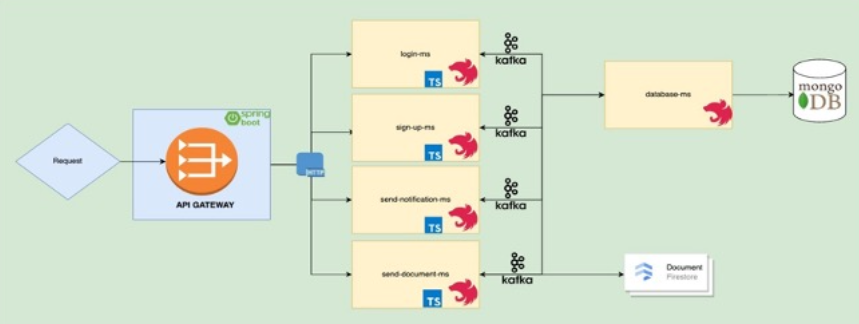
\includegraphics[scale=0.44]{assets/application-arch}
    \label{fig:application-arch}
    \tiny
    \sourcemedaddy
\end{figure}


\section{Requisitos funcionais e não funcionais}

\chapter{CRIAÇÃO DOS AMBIENTES DE DESENVOLVIMENTO}

\section{Introdução}

Este capítulo aborda o processo de criação e configuração dos ambientes e infraestruturas
necessárias para o desenvolvimento do protótipo de aplicação, incluindo o repositório no GitHub,
configuração do NestJS para monorepo, e a criação dos containers Docker e Docker Compose.
Cada uma dessas etapas é detalhada, com foco em suas contribuições para a construção de uma
arquitetura de micro serviços e mensageria, conforme modelado pelo C4 Model.

\section{Configuração do Supabase}

Conforme mencionado anteriormente, o Supabase é uma plataforma open-source que
simplifica a criação e gestão de componentes relacionados a bancos de dados e autenticação.
Ao iniciar um projeto, o Supabase configura automaticamente um banco de dados PostgreSQL
como estrutura base.

Adicionalmente, a plataforma oferece suporte à Row Level Security (RLS), que além de
assegurar a autenticação dos usuários, possibilita a configuração de autorizações, determinando
o nível de acesso (roles) de cada usuário conforme sua função ou permissão.
Outra grande vantagem sobre o Supabase, é a facilidade, pois para criar um projeto com
eles, podemos apenas acessar o link (https://supabase.com).

Um exemplo de criação de um projeto utilizando supabase:

\begin{figure}[!ht]
    \centering
    \caption{Criando o projeto no Supabase}
    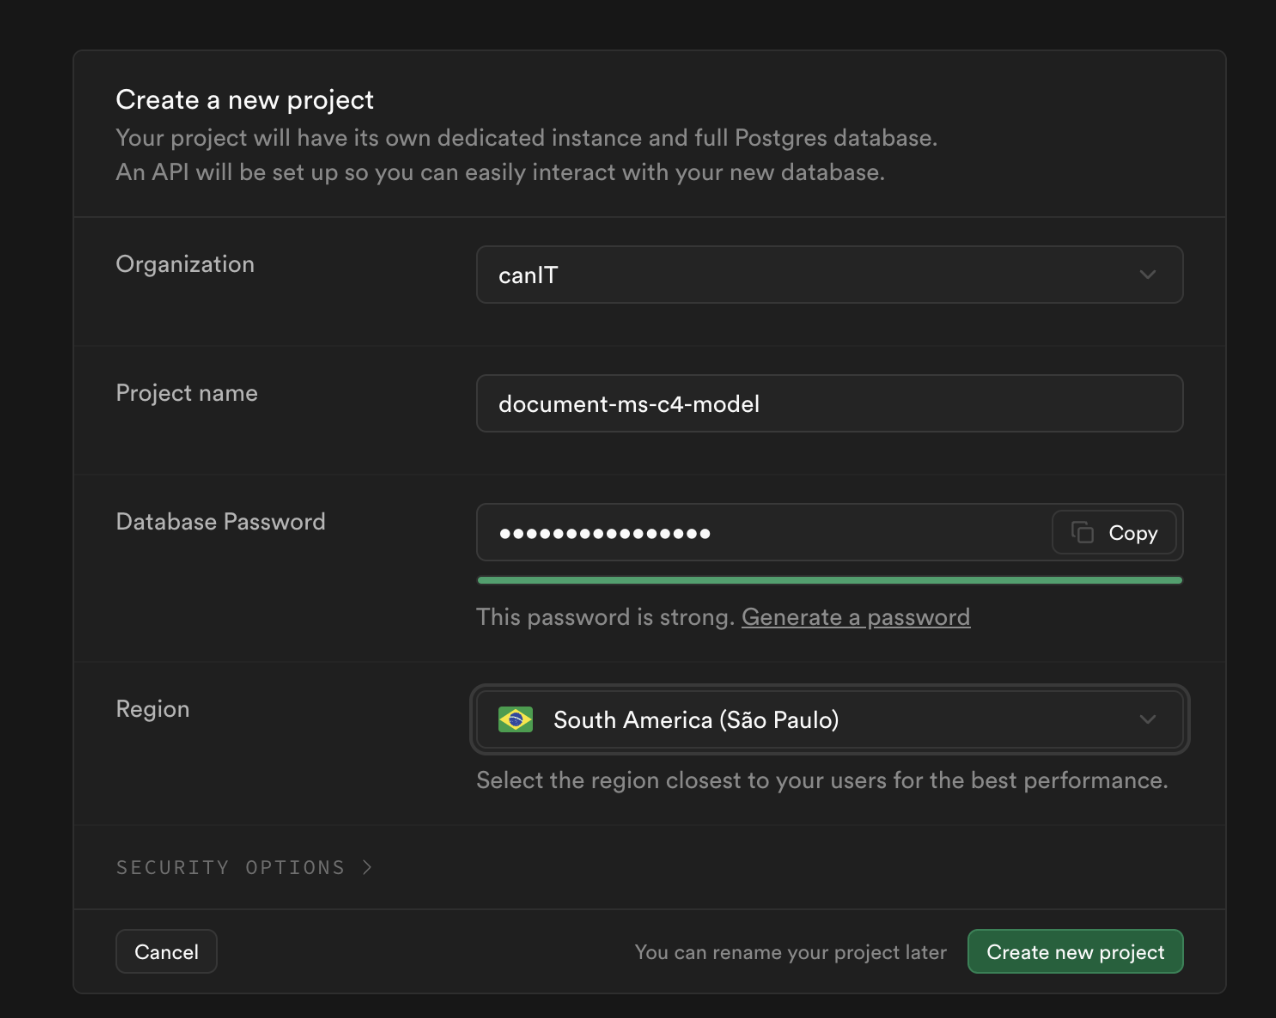
\includegraphics[scale=0.44]{assets/create-new-project}
    \label{fig:create-new-project}
    \tiny
    \sourcemedaddy
\end{figure}

Após a criação, temos um período de configuração, costuma demorar menos que 5
minutos, é redirecionado para essa página:

\begin{figure}[!ht]
    \centering
    \caption{Pendente de criação}
    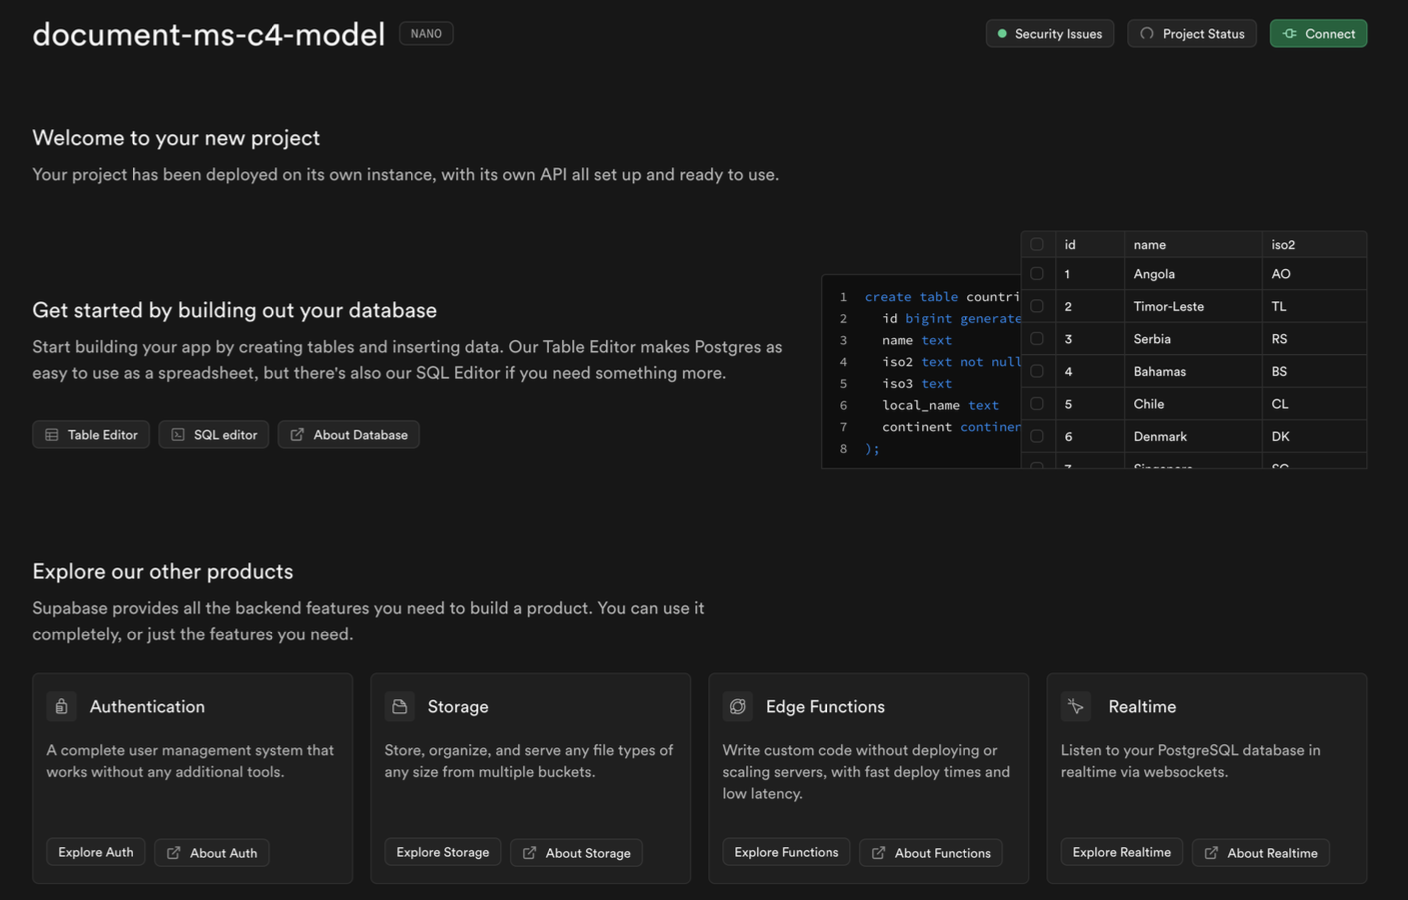
\includegraphics[scale=0.44]{assets/pending-creation}
    \label{fig:pending-creation}
    \tiny
    \sourcemedaddy
\end{figure}

Primeiro usuário criado no painel do Supabase:

\begin{figure}[!ht]
    \centering
    \caption{Pendente de criação}
    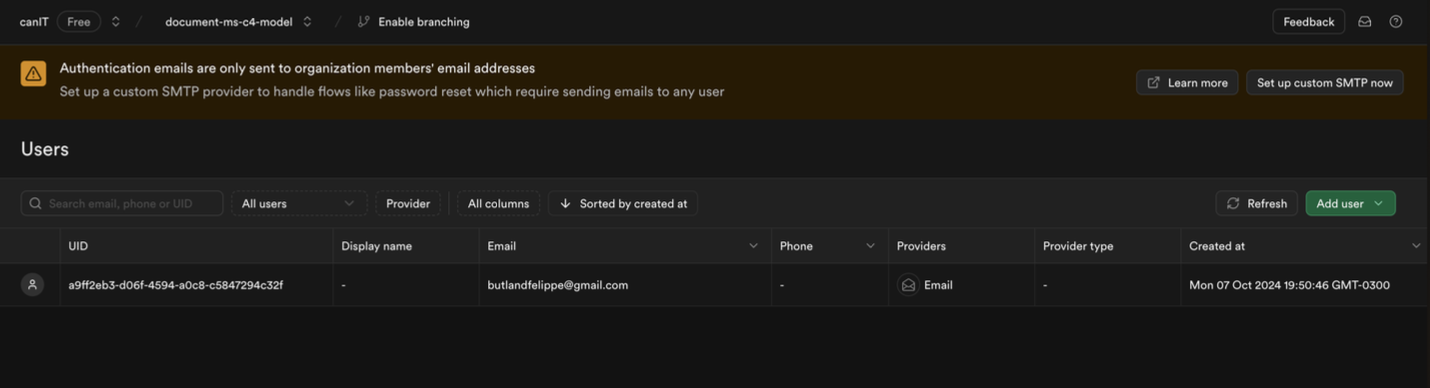
\includegraphics[scale=0.44]{assets/first-user}
    \label{fig:first-user}
    \tiny
    \sourcemedaddy
\end{figure}

\section{Criação de Repositório no GitHub}

A primeira etapa no processo de desenvolvimento é a criação do repositório onde o código-fonte será armazenado e versionado. O GitHub foi escolhido como plataforma de controle de versões, pois oferece integração com diversas ferramentas de CI/CD e uma ampla comunidade de desenvolvedores. A seguir estão os passos para a criação do repositório:

\begin{enumerate}
    \item Acesse o GitHub e faça login com suas credenciais.
    \item No canto superior direito da página inicial, clique em “+” e selecione a opção "New repository".
    \item Preencha as informações do repositório:
    \begin{itemize}
        \item \textbf{Repository name:} Nome do repositório (ex: "document-sharing-microservices").
        \item \textbf{Description:} Descrição breve do repositório (ex: "Protótipo de aplicação de envio de documentos modelado com C4, utilizando micro serviços e mensageria.").
        \item \textbf{Public/Private:} Selecione se o repositório será público ou privado.
        \item \textbf{Initialize this repository with:} Marque a opção "Add a README file" para inicializar o repositório com um arquivo README.
    \end{itemize}
    \item Clique em “Create repository”.
\end{enumerate}

Após a criação do repositório, o código fonte poderá ser versionado e colaborado com outras equipes utilizando Git.

\section{Configuração do NestJS para Monorepo e API Gateway}

O NestJS é um framework para desenvolvimento de aplicações backend utilizando Node.js e TypeScript. Para este projeto, a configuração de um monorepo utilizando NestJS facilita o gerenciamento de múltiplos micro serviços em uma única base de código, proporcionando escalabilidade e modularidade. Além disso, um API Gateway foi desenvolvido para atuar como a entrada centralizada para as requisições direcionadas aos diferentes micro serviços. O uso do API Gateway simplifica a comunicação entre o cliente e os serviços, permitindo uma melhor organização e gestão das requisições.

\subsection{Configuração do Monorepo}
Os passos para a configuração do monorepo são os seguintes:

\begin{enumerate}
    \item Instale o NestJS CLI globalmente utilizando o comando:
    \begin{verbatim}
    npm i -g @nestjs/cli
    \end{verbatim}
    \item Crie um novo projeto NestJS com suporte a monorepo, utilizando o comando:
    \begin{verbatim}
    nest new project-name --monorepo
    \end{verbatim}
    \item Durante a criação, selecione as opções desejadas para o gerenciamento de pacotes e outros aspectos do projeto.
    \item Navegue até o diretório do projeto e verifique a estrutura de pastas. O NestJS criará uma estrutura base contendo a pasta \texttt{apps}, que armazenará os micro serviços, e a pasta \texttt{libs}, que conterá os módulos compartilhados entre os micro serviços.
    \item Crie um novo micro serviço com o comando:
    \begin{verbatim}
    nest generate app microservice-name
    \end{verbatim}
    \item Para garantir que os micro serviços estejam corretamente configurados, execute o comando:
    \begin{verbatim}
    npm run start:dev
    \end{verbatim}
    Este comando iniciará o serviço em ambiente de desenvolvimento.
\end{enumerate}

\subsection{Desenvolvimento do API Gateway}
Para atuar como a entrada centralizada para as requisições, o API Gateway foi implementado no mesmo monorepo. Os passos para a configuração do API Gateway são os seguintes:

\begin{enumerate}
    \item Navegue até o diretório do projeto e crie uma nova aplicação para o API Gateway:
    \begin{verbatim}
    nest generate app api-gateway
    \end{verbatim}
    \item Instale as dependências necessárias, como o \texttt{@nestjs/microservices} para habilitar a comunicação entre micro serviços.
    \item Configure os controladores no API Gateway para encaminhar as requisições para os serviços apropriados. Utilize decorators como \texttt{@Get()}, \texttt{@Post()} etc., para definir as rotas.
    \item Implemente a lógica de balanceamento de carga, se necessário, utilizando a biblioteca \texttt{@nestjs/microservices} para garantir que as requisições sejam distribuídas de forma equitativa entre instâncias de micro serviços.
\end{enumerate}

\subsection{Suporte à Escalabilidade}
O API Gateway proporciona escalabilidade de diversas maneiras:

\begin{itemize}
    \item \textbf{Balanceamento de Carga}: Permite distribuir as requisições entre várias instâncias de um micro serviço, evitando sobrecargas e melhorando a disponibilidade.

    \item \textbf{Roteamento Dinâmico}: Facilita a adição ou remoção de serviços, permitindo que novos recursos sejam acessados rapidamente sem a necessidade de alterar a lógica de roteamento.

    \item \textbf{Escalabilidade Horizontal}: Cada micro serviço pode ser escalado independentemente, permitindo que a infraestrutura cresça conforme a demanda sem impactar os demais serviços.
\end{itemize}

\subsection{Considerações Finais}
A configuração do NestJS em um monorepo e a implementação do API Gateway proporcionam uma base sólida para o desenvolvimento de aplicações escaláveis e modulares. Essa arquitetura não apenas melhora a comunicação entre os micro serviços, mas também oferece flexibilidade para a adaptação a mudanças nas necessidades do negócio. A integração do API Gateway garante que o sistema possa crescer de forma organizada, permitindo uma resposta ágil às demandas do mercado e dos usuários.

\section{Criação do Docker e Docker Compose}

O Docker é utilizado para empacotar as aplicações em containers, garantindo consistência entre os ambientes de desenvolvimento e produção. O Docker Compose permite orquestrar múltiplos containers, facilitando a comunicação entre os micro serviços e o banco de dados. Para configurar o Docker e o Docker Compose para este projeto, siga os passos abaixo:

\subsection{Criação do Dockerfile}
Cada micro serviço criado no NestJS precisará de um arquivo Dockerfile para definir como o container será construído. O exemplo a seguir mostra a configuração básica de um Dockerfile para um micro serviço NestJS:

\begin{verbatim}
FROM node:16
WORKDIR /usr/src/app
COPY package*.json ./
RUN npm install
COPY . .
EXPOSE 3000
CMD ["npm", "run", "start:prod"]
\end{verbatim}

\subsection{Criação do docker-compose.yml}
O arquivo \texttt{docker-compose.yml} será utilizado para definir e orquestrar os containers dos micro serviços e dos componentes auxiliares, como bancos de dados e filas de mensagens. Um exemplo básico de configuração para o Docker Compose é apresentado a seguir:

\begin{verbatim}
version: '3.8'
services:
  kafka:
    image: confluentinc/cp-kafka:latest
    depends_on:
      - zookeeper
    ports:
      - 29092:29092
    environment:
      KAFKA_BROKER_ID: 1
      KAFKA_ZOOKEEPER_CONNECT: zookeeper:2181
      KAFKA_ADVERTISED_LISTENERS: PLAINTEXT://kafka:9092
      KAFKA_INTER_BROKER_LISTENER_NAME: PLAINTEXT
      KAFKA_OFFSETS_TOPIC_REPLICATION_FACTOR: 1
  kafka_ui:
    image: provectuslabs/kafka-ui:latest
    depends_on:
      - kafka
    ports:
      - 8080:8080
    environment:
      KAFKA_CLUSTERS_0_ZOOKEEPER: zookeeper:2181
      KAFKA_CLUSTERS_0_NAME: local
      KAFKA_CLUSTERS_0_BOOTSTRAPSERVERS: kafka:9092
volumes:
  mongodb_data_container:
\end{verbatim}

Este arquivo define o serviço da aplicação e do Kafka.

\subsection{Desafios de Rede com Docker}

Um dos principais desafios ao usar o Docker em um ambiente onde o banco de dados Supabase está localizado em uma rede diferente da rede Docker é a comunicação entre os containers e o banco de dados externo. Aqui estão alguns problemas que surgiram durante a configuração e as soluções aplicadas:

\begin{itemize}
    \item \textbf{Conectividade de Rede}: Inicialmente, os micro serviços não conseguiam se conectar ao Supabase devido à falta de configuração das variáveis de ambiente que definem as credenciais e a URL do banco de dados. A solução foi garantir que cada serviço no Docker recebesse as variáveis de ambiente corretas, utilizando o arquivo \texttt{docker-compose.yml} para passar essas informações, por exemplo:
    \begin{verbatim}
    environment:
      SUPABASE_URL: <url_do_supabase>
      SUPABASE_ANON_KEY: <chave_anonima>
    \end{verbatim}

    \item \textbf{Configuração de Redes Docker}: A comunicação entre os micro serviços e as filas de mensagens, como o Kafka, também apresentou dificuldades. Para resolver isso, foi criada uma rede personalizada no Docker Compose, permitindo que os serviços se comunicarem entre si e com o Supabase. A configuração foi realizada da seguinte forma:
    \begin{verbatim}
    networks:
      app-network:
        driver: bridge
    \end{verbatim}

    E cada serviço foi adicionado a esta rede:
    \begin{verbatim}
    services:
      kafka:
        networks:
          - app-network
      microservice:
        networks:
          - app-network
    \end{verbatim}

    \item \textbf{Latência de Rede}: A comunicação entre os containers e o Supabase pode introduzir latência, especialmente sob alta carga de tráfego. Foi implementado um mecanismo de retry e timeouts nas requisições feitas ao banco, garantindo que as operações críticas fossem executadas mesmo diante de instabilidades temporárias.

    \item \textbf{Perda de Conexões}: Em situações de reinicialização de containers, houve momentos em que as conexões com o banco de dados foram perdidas. Para mitigar esse problema, foi utilizado um padrão de reconexão automática nos micro serviços, que tentam reconectar-se ao Supabase até que a conexão seja restabelecida.
\end{itemize}

Esses desafios exigem uma configuração cuidadosa da rede e testes rigorosos para garantir que a comunicação entre os micro serviços e o Supabase seja confiável e eficiente. A implementação de práticas de robustez, como retries e configuração de variáveis de ambiente, ajudou a minimizar problemas de conectividade e latência, garantindo que o sistema como um todo funcione conforme o esperado.

\section{Configuração do Kafka e Zookeeper}

O Apache Kafka é uma plataforma de streaming de eventos que permite a construção de pipelines de dados em tempo real e aplicações de streaming. Para o funcionamento adequado do Kafka, é necessário o uso do Zookeeper, que é responsável por gerenciar a configuração do Kafka e o estado dos brokers. A configuração correta de ambos é essencial para garantir a resiliência e o desempenho do sistema. Abaixo, detalharemos a configuração dos serviços Kafka e Zookeeper, bem como os problemas comuns relacionados à latência e à perda de mensagens.

\subsection{Configuração do Zookeeper}
O Zookeeper deve ser configurado adequadamente para garantir que o Kafka funcione corretamente. No arquivo \texttt{docker-compose.yml}, o Zookeeper pode ser definido como um serviço separado, conforme exemplificado abaixo:

\begin{verbatim}
  zookeeper:
    image: wurstmeister/zookeeper:3.4.6
    ports:
      - 2181:2181
    environment:
      ZOOKEEPER_CLIENT_PORT: 2181
      ZOOKEEPER_TICK_TIME: 2000
\end{verbatim}

O parâmetro \texttt{ZOOKEEPER\_TICK\_TIME} define a frequência com que o Zookeeper envia notificações aos seus clientes e deve ser ajustado conforme a necessidade do sistema.

\subsection{Configuração do Kafka}
No arquivo \texttt{docker-compose.yml}, o Kafka é configurado para se conectar ao Zookeeper e definir as opções de replicação e comunicação entre brokers. A configuração apresentada anteriormente inclui as seguintes variáveis de ambiente:

\begin{verbatim}
  KAFKA_ZOOKEEPER_CONNECT: zookeeper:2181
  KAFKA_ADVERTISED_LISTENERS: PLAINTEXT://kafka:9092
  KAFKA_INTER_BROKER_LISTENER_NAME: PLAINTEXT
  KAFKA_OFFSETS_TOPIC_REPLICATION_FACTOR: 1
\end{verbatim}

- \textbf{KAFKA\_ZOOKEEPER\_CONNECT:} Define a conexão do Kafka com o Zookeeper.
- \textbf{KAFKA\_ADVERTISED\_LISTENERS:} Especifica os listeners disponíveis para os clientes se conectarem.
- \textbf{KAFKA\_INTER\_BROKER\_LISTENER\_NAME:} Determina o listener a ser usado para a comunicação entre brokers.
- \textbf{KAFKA\_OFFSETS\_TOPIC\_REPLICATION\_FACTOR:} Define o fator de replicação dos tópicos de offsets, que deve ser maior que 1 em produção para garantir alta disponibilidade.

\subsection{Problemas de Latência}
Um dos desafios ao trabalhar com Kafka é a latência. A latência pode ser causada por diversos fatores, como a configuração inadequada do número de partições, a replicação excessiva de dados ou a largura de banda insuficiente. Para mitigar a latência, recomenda-se:

\begin{itemize}
    \item Otimizar o número de partições para permitir um balanceamento adequado de carga.
    \item Ajustar as configurações de flush e a quantidade de memória disponível para o Kafka.
    \item Monitorar a rede e a infraestrutura para identificar gargalos.
\end{itemize}

\subsection{Perda de Mensagens}
A perda de mensagens é outro problema crítico em sistemas que utilizam Kafka. Isso pode ocorrer devido a configurações de replicação inadequadas ou falhas de broker. Para minimizar o risco de perda de mensagens, as seguintes práticas são recomendadas:

\begin{itemize}
    \item Configurar o fator de replicação dos tópicos para um valor maior que 1.
    \item Usar o modo de produção \texttt{acks=all} para garantir que todas as réplicas confirmem a gravação antes de considerar a mensagem como recebida.
    \item Implementar um sistema de monitoramento para detectar falhas rapidamente e garantir a recuperação adequada.
\end{itemize}

A correta configuração do Kafka e do Zookeeper, juntamente com a consideração dos problemas de latência e perda de mensagens, é essencial para garantir um sistema robusto e confiável de micro serviços.

\section{Arquitetura de Micro Serviços e Mensageria}

Neste projeto, a arquitetura de micro serviços é baseada em múltiplos serviços indepen-
dentes que se comunicam por meio de eventos assíncronos utilizando mensageria. A solução
de mensageria escolhida foi Kafka, adequado para sistemas que requerem alta escalabilidade e
comunicação entre serviços desacoplados.

A comunicação entre micro serviços será modelada utilizando o C4 Model, uma aborda-
gem que divide a arquitetura em quatro níveis: contexto, containers, componentes e código. Este
modelo permite uma visualização clara da interação entre os micro serviços e seus componentes,
como a fila de mensagens que gerencia o envio e recebimento de documentos.

\section{Configuração com C4 model}

O C4Builder é uma ferramenta que facilita a criação de configurações de projeto utilizando C4 model, essencial para a criação de diagramas arquiteturais, que ajudam na documentação e visualização da estrutura do sistema. No contexto deste projeto, o C4Builder foi utilizado para modelar a arquitetura dos micro serviços, utilizando o C4 Model para representar a interação entre os diferentes componentes do sistema de envio de documentos.

Durante a configuração inicial do repositório, o C4Builder auxiliou na definição clara da estrutura de micro serviços e na organização do código, contribuindo para o planejamento e a organização do desenvolvimento. Especificamente, o C4Builder ajudou nas seguintes etapas:

\begin{enumerate}
    \item \textbf{Definição do Diagrama de Contexto:} O C4Builder permitiu a criação de um diagrama de contexto, onde foram mapeados os principais atores do sistema, como usuários e sistemas externos, e suas interações com o sistema de envio de documentos. Esse diagrama ajudou a entender melhor os requisitos e os pontos de integração com outros sistemas e serviços.

    \item \textbf{Planejamento da Arquitetura de Containers:} Utilizando o C4Builder, foi possível projetar o diagrama de containers, representando a divisão do sistema em micro serviços, banco de dados, fila de mensagens e outros componentes importantes. Esse planejamento ajudou a visualizar como cada parte do sistema seria implementada e como elas interagiriam.

    \item \textbf{Mapeamento dos Componentes do Sistema:} O C4Builder também facilitou o mapeamento dos componentes dentro de cada container, ajudando a definir claramente as responsabilidades e interações entre os serviços, como o serviço de autenticação, processamento de documentos e envio de notificações.
\end{enumerate}

Com o uso do C4Builder, foi possível criar uma base sólida para o desenvolvimento inicial do repositório, assegurando que a estrutura do sistema fosse bem definida antes da implementação prática dos micro serviços e demais componentes. O C4Builder auxiliou na visualização da arquitetura do sistema, o que permitiu uma configuração mais organizada e orientada para as melhores práticas de desenvolvimento em micro serviços.


\section{Casos de Sucesso em Mensageria e Microserviços}

A adoção de arquiteturas baseadas em microserviços e mensageria tem se tornado cada vez mais comum entre startups e grandes empresas de tecnologia. Essa abordagem permite maior escalabilidade, flexibilidade e resiliência em sistemas complexos. As microservices são implementados como serviços independentes que podem ser desenvolvidos, implantados e escalados de forma autônoma, enquanto a mensageria garante a comunicação entre esses serviços de maneira eficiente. A seguir, apresentamos alguns casos de sucesso notáveis que ilustram a eficácia dessa arquitetura.

\subsection{Startups}
Muitas startups têm encontrado na mensageria e na arquitetura de microserviços um caminho para acelerar o desenvolvimento e a entrega de suas aplicações.

\begin{itemize}
    \item \textbf{Slack}: A plataforma de comunicação em equipe Slack utiliza uma arquitetura de microserviços que lhe permite escalar rapidamente e atender a milhões de usuários simultaneamente. A mensageria desempenha um papel crucial em sua infraestrutura, permitindo a comunicação assíncrona entre os diferentes serviços. Cada funcionalidade, como mensagens diretas, canais e notificações, é gerenciada por serviços distintos que se comunicam por meio de uma fila de mensagens, garantindo que as mensagens sejam entregues de forma confiável, mesmo em casos de alta carga.

    \item \textbf{Netflix}: Embora já seja uma gigante do setor, a Netflix começou como uma startup e rapidamente cresceu, adotando microserviços para gerenciar sua plataforma de streaming. O uso de uma arquitetura de mensageria robusta permite à Netflix implementar novos recursos rapidamente, escalar sua plataforma globalmente e garantir uma experiência de usuário fluida. A Netflix desenvolveu seu próprio sistema de mensageria, chamado \textit{Kafka}, que é usado para gerenciar bilhões de eventos por dia, permitindo a coleta e análise de dados em tempo real sobre o comportamento dos usuários.

    \item \textbf{Airbnb}: O Airbnb é outro exemplo de startup que implementou microserviços para gerenciar sua plataforma de aluguel de imóveis. Ao adotar uma arquitetura de microserviços, o Airbnb conseguiu isolar diferentes funcionalidades, como reservas, pagamentos e avaliações, permitindo que equipes diferentes trabalhassem em paralelo. A mensageria ajuda a garantir que as interações entre esses serviços sejam eficientes, minimizando a latência e melhorando a experiência do usuário.
\end{itemize}

\subsection{Big Techs}
As grandes empresas de tecnologia também utilizam mensageria e microserviços para resolver desafios complexos e atender à demanda de seus produtos.

\begin{itemize}
    \item \textbf{Amazon}: A Amazon utiliza uma arquitetura de microserviços em sua plataforma de comércio eletrônico, permitindo que diferentes partes do sistema operem de forma independente. Isso facilita o lançamento de novos produtos e recursos sem impactar toda a plataforma. A mensageria é uma parte fundamental de sua infraestrutura, facilitando a comunicação entre serviços e garantindo que eventos como pedidos e pagamentos sejam processados de forma eficiente e segura. A Amazon Web Services (AWS) também fornece uma variedade de serviços de mensageria, como o Amazon SQS e o Amazon SNS, que ajudam outras empresas a implementar soluções baseadas em mensageria.

    \item \textbf{Google}: O Google implementa microserviços em diversos produtos, incluindo o Google Cloud Platform. A empresa utiliza sistemas de mensageria como o Pub/Sub para permitir a comunicação entre serviços e gerenciar a troca de dados em tempo real, apoiando aplicações escaláveis e de alta performance. A arquitetura de microserviços do Google possibilita que equipes autônomas desenvolvam e implantem serviços rapidamente, aumentando a agilidade no desenvolvimento e a capacidade de resposta às necessidades dos usuários.

    \item \textbf{Uber}: O Uber adota uma arquitetura de microserviços para gerenciar sua plataforma de transporte, que envolve múltiplos serviços que lidam com reservas, pagamentos, geolocalização e muito mais. A mensageria permite que os diferentes componentes do sistema se comuniquem eficientemente, resultando em tempos de resposta rápidos e em uma experiência de usuário otimizada. A arquitetura do Uber é altamente distribuída, permitindo que a empresa lide com a demanda em tempo real e escale sua infraestrutura conforme necessário.
\end{itemize}

\subsection{Considerações Finais}
O uso de mensageria e microserviços tem sido fundamental para o sucesso de diversas startups e grandes empresas de tecnologia. Essas arquiteturas oferecem vantagens significativas em termos de escalabilidade, resiliência e capacidade de resposta a mudanças no mercado. Além disso, a capacidade de implantar e escalar serviços independentemente permite que as organizações inovem rapidamente e respondam às demandas dos usuários de maneira eficiente.

À medida que mais organizações adotam essa abordagem, espera-se que novas inovações e casos de uso continuem a emergir, solidificando ainda mais a importância da mensageria e dos microserviços na engenharia de software moderna. A tendência é que a combinação de mensageria e microserviços se torne cada vez mais prevalente, com empresas buscando maneiras de otimizar seus processos e melhorar a experiência do cliente por meio da tecnologia.




\bibliography{references/export}

% Glossário
 %\chapter*{GLOSSÁRIO}
\addcontentsline{toc}{chapter}{GLOSSARIO}
\begin{itemize}
    \item DF (Dataframe): Um tipo de tabela estruturada para processamento e análise de dados (semelhante ao Excel) e comum em sistemas utilizando o Spark e a biblioteca Pandas
\end{itemize}

% Elemento opcional. Consiste em uma lista de palavras ou expressões técnicas de uso restrito ou de sentido obscuro, utilizadas no texto, acompanhadas das respectivas definições.

% Apêndice
 %\chapter*{APÊNDICE}
\addcontentsline{toc}{chapter}{APÊNDICE}
Elemento opcional. Texto ou documento elaborado pelo autor, que serve de fundamentação, comprovação e ilustração.

% Anexo
 %\chapter*{ANEXO}
\addcontentsline{toc}{chapter}{ANEXO}
Elemento opcional. Texto ou documento não elaborado pelo autor, que serve de fundamentação, comprovação e ilustração.

% Índice
 %\chapter*{ÍNDICE}
\addcontentsline{toc}{chapter}{ÍNDICE}
Elemento opcional. Consiste em uma lista de autor, título ou assunto em ordem alfabética ou sistemática (por classes, numérica ou cronológica) que remete para as informações contidas no texto.


\end{OnehalfSpace}
\end{document}
